\documentclass{article}
\usepackage[utf8]{inputenc}

\title{Conversion de coordonnées image vers plan de jeu}
\date{Mars 2019}

\usepackage{natbib}
\usepackage{graphicx}
\usepackage{amsmath} 

\begin{document}

\maketitle

\section{Théorie}

On considérera dans la suite la géométrie de la \ref{fig1} pour la position et l'orientation de la caméra.

\begin{figure}[h!]
\centering
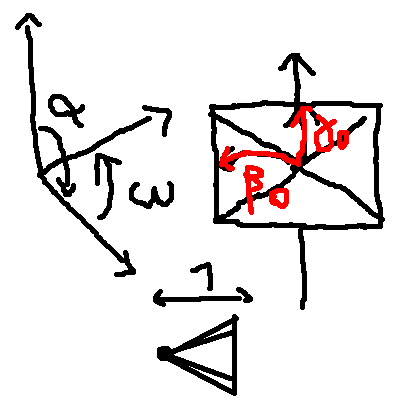
\includegraphics[scale=0.5]{camera.png}
\caption{Les coordonnées image.}
\label{fig1}
\end{figure}

On part d'une image avec des coordonnées exprimées en pixels, la position (0,0) étant en haut à gauche de l'image (\ref{fig2}). Il sera important dans la suite de considérer si l'image est retournée ou pas (la gauche de l'image correspondrait à la droite de la caméra).

\begin{figure}[h!]
\centering
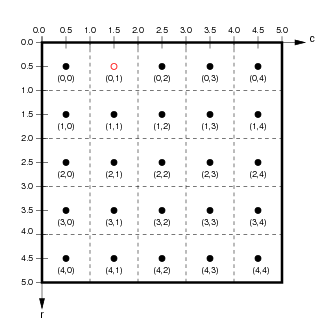
\includegraphics[scale=0.5]{image.png}
\caption{Les coordonnées image.}
\label{fig2}
\end{figure}


On va chercher à convertir cette image en coordonnées pixel en coordonnées sur un plan image fictif. Pour cela, on supposera que la caméra se situe à une distance 1 du plan. Ainsi, la distance maximale au centre de la bijection de l'image sur le plan image est en $\tan(\beta_0)$ et $\tan(\gamma_0)$. Ainsi, on utilisera la conversion décrite par (\ref{conversion}).

\begin{equation}
\label{conversion}
\left\{
    \begin{array}{ll}
        x = \tan(\beta_0)(\frac{2u}{resoX}-1)\\
        z = \tan(\gamma_0)(\frac{2v}{resoZ} -1)
    \end{array}
\right.
\end{equation}
resoX étant le nombre de pixels en x et resoY respectivement en y, u et v étant les coordonnées sur l'image.

On peut interpréter la position sur le plan image comme un vecteur directeur de direction à partir de la caméra. On veut convertir cette direction dans le repère de la table et non plus celui de la caméra. Pour cela on va effectuer deux rotations successives correspondant aux angles $\gamma_0$ et $\beta_0$ de la caméra (\ref{rotation}).

\begin{equation}
\label{rotation}
\vec{P_{rot}} =
\begin{pmatrix}
\cos(\omega) & \sin(\omega)\cos(\alpha) & \sin(\omega)\sin(\alpha) \\
\sin(\omega) & \cos(\omega)\cos(\alpha) & \cos(\omega)\sin(\alpha)\\
0 & \sin(\alpha) & \cos(\alpha)\\
\end{pmatrix}
\quad
\vec{P_{cam}}
\end{equation}

A présent que l'on connaît la direction dans le repère du plan de jeu, on va calculer le point d'intersection de la droite partant de la caméra dans la direction $\vec{P_{rot}}$ avec le plan situé à une hauteur $h$ de la caméra (Cette hauteur étant à adapter en fonction de la nature de la cible, robot ou palet). Ces coordonnées s'obtiennent selon \ref{intersection}.

\begin{equation}
\label{intersection}
\left\{
    \begin{array}{ll}
        x = h * \frac{P_{rotX}}{P_{rotZ}}\\
        y = h * \frac{P_{rotY}}{P_{rotZ}}
    \end{array}
\right.
\end{equation}

Il ne reste plus qu'à éventuellement tenir compte d'une translation de la caméra par rapport à l'origine fixée quelque part sur la table.


\end{document}
